\section{Introduction}
A major long-term goal of robotics research is the introduction of intelligent household robots.
Such robots would face complex tasks, such as setting
dinner tables and doing laundry. Planning for these long-horizon tasks is infeasible
using only motion planning due to the sheer number of steps involved, making apparent the need
for a hierarchical system of reasoning.

Recent methods for hierarchical planning focus on the intersection of high level task planning
and low level motion planning. In this framework, the (classical) task planner produces
a symbolic plan containing a sequence of actions to reach a goal
state, and an interface layer refines this plan by sampling concrete values for
the abstract symbols, thus grounding the plan. A central challenge in building such
an interface layer is designing good distributions from which to sample
values for the symbolic plan parameters.

\begin{figure}[h]
  \centering
    \noindent
    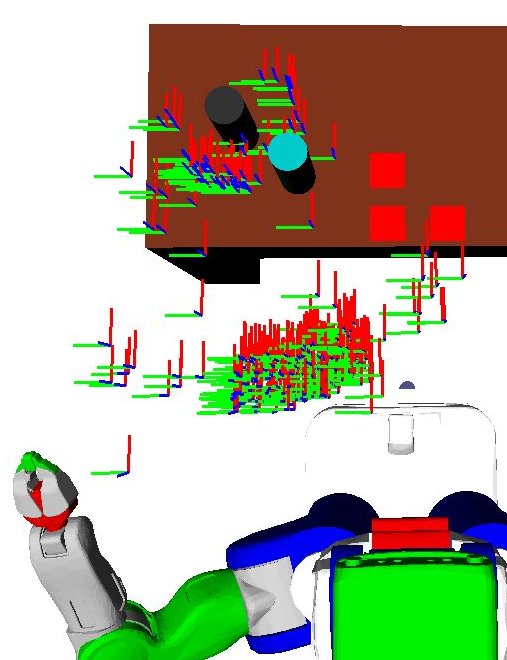
\includegraphics[scale=0.2]{images/move_grasp.png}\hspace{10 mm}
    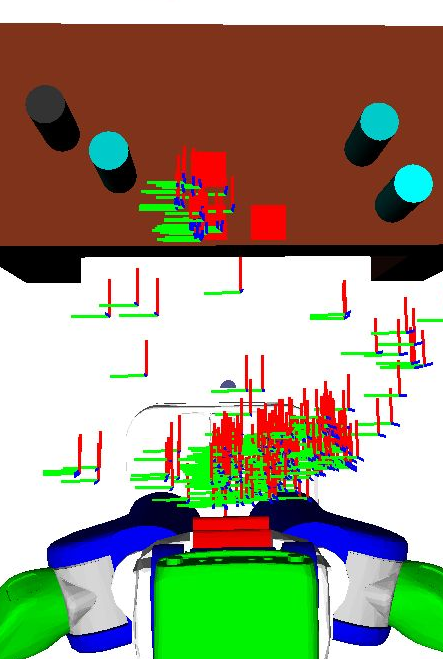
\includegraphics[scale=0.2]{images/move_putdown.png}
  \caption{Screenshots showing some distributions learned by our system in one experimental
    setup. The robot is tasked with grasping the black cylinder and putting it down on the
    central red square. The left image shows learned base motion and grasping distributions,
    and the right shows learned base motion and putdown distributions. The grasp distribution
    properly learned to avoid the region close to the blue obstruction. We sample from these distributions
    to refine the high level plan, rather than relying on hand-coded ones.}
  \label{fig:cover}
\end{figure}

Our work improves directly upon recent approaches to task and motion planning.
A key limitation of these systems is that they typically rely on hand-coded
sampling distributions to instantiate continuous values for grounding a symbolic plan.
These distributions often rely on
geometric information about the object of interest, surrounding objects, and overall
environment. This restriction has several negative implications: the parameters of the
hand-coded distributions must be fine-tuned when running the system in a new setting, and the
resulting refinement distributions are discretized, lacking robustness.

Our main contribution is a reinforcement learning approach to find good proposal
distributions for symbolic plan refinement, using rollouts. We take inspiration
from the work of Zhang and Dietterich, who explored applying reinforcement learning
to planning problems in a job shop scheduling setting. Using methods adapted from
Zucker et al., who train a configuration space sampler for motion planning
using features of the discretized workspace, we train a policy that
determines how to sample values for plan symbols, using $TD(\lambda)$ with linear function
approximation. Our approach allows
the learned distributions to be continuous, robust to changes in the environment, and
trainable for any experimental setting, eliminating the need for hand-tuning distribution parameters.

A second contribution of our work is randomized refinement, a novel refinement strategy
which maintains at all times a set of values for all symbolic plan variables, then randomly
resamples one whose current instantiation is causing a failure.
This refinement algorithm allows for a clear formulation of the reinforcement
learning system and naturally guides variable resampling intelligently, so that better
sampling distributions can be learned more easily for complex environments.

Our implementation builds directly off the system presented by Srivastava et al.
They propose a complete backtracking search algorithm for refining
the symbolic plan skeleton into a set of collision-free trajectories using motion planning.
If a motion planning feasible refinement is not found within the resource limit,
symbolic error information is propagated back to the task planner, and a new symbolic plan is produced.
The system uses an off-the-shelf classical task planner and motion planner, both as black boxes.
We evaluate our approach in a variety of test environments involving complicated grasp and putdown
actions with obstructions and base motion. Our experimental results demonstrate
comparable to improved performance for both motion planning time and number of calls to
the motion planner, when compared to the hand-coded distributions used in the original system.